\chapter{Related work}
There already exist some examples of blockchains being used in the energy market.  

Using blockchain in the energy market was first proposed by Mihaylov et al. \cite{NRGcoin_Mihaylov}. NRGcoin was introduced as digital currency for buying and selling energy through smart contracts. However, the transactions are not done in a P2P approach. 
 
There are several companies emerging, that are developed for P2P energy trading. Three of these, all entering the market in 2016 or later, will be further discussed. 

%https://publik.tuwien.ac.at/files/publik_265619.pdf

\section{Brooklyn Microgrid} \label{Brooklyn}
The Brooklyn Microgrid is a project owned by LO3, where some neighbors in Brooklyn, New York trade energy  \cite{bm101}. This is done in a peer-to-peer manner, over the blockchain, thus removing the middleman. Residents who have installed solar panels on their roof tops, can sell any excess energy to their neighbors. The first transaction occurred in April 2016, and is \cite{exergy, motherboard_bm} the first ever energy transaction made on a blockchain. 

The company started working with the public blockchain Ethereum \cite{medium_bm, motherboard_bm}, which was the first blockchain to make a non-financial transaction. However, they quickly realized that this was not a feasible solution, and decided to make their own, private blockchain.

The microgrid was developed by the Siemens Digital Grid Division, while the blockchain platform was developed by LO3 Energy. 
Each participant in the project has a meter installed. These meters communicate with each other, and other smart devices. Furthermore, they measure the energy production and consumption. The key factor, however, is that these meters form the blockchain \cite{medium_bm, hbr_grid}. Transactions from each meter is stored on the blockchain, while all meters contribute with the computational power necessary to run the blockchain and validate the transactions. 

Mengelkamp et al. \cite{Brooklyn_Mengelkamp} presented a case study of the Brooklyn Microgrid. The project consists of both a virtual platform and a physical microgrid. The microgrid is built in parallel with the existing grid, and is able to uncouple from the traditional gird in case of power outages. The virtual platform is the technical infrastructure, and runs a private blockchain. The virtual layer is where all the information of the network is transferred. 

\begin{figure}[htb]
    \centering
    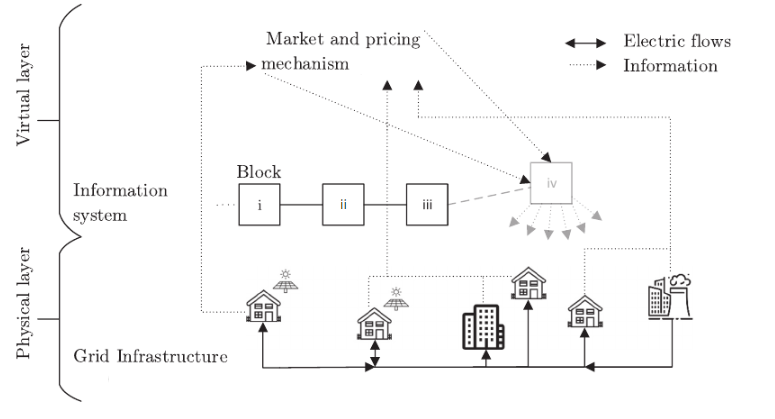
\includegraphics[width=1\textwidth]{Images/bm}
    \caption{High-level topology of the Brooklyn Microgrid \cite{Brooklyn_Mengelkamp}.}
    \label{fig:bm}
\end{figure}
 

\section{NAD Grid}
NAD Grid is a platform for peer-to-peer energy transactions over the blockchain, based in Silicon Valley \cite{nad_youtube}. The company focuses on reducing carbon footprint through their Selective Sourcing technology \cite{nad}.

The software platform is built upon the physical grid, and they aim to partner with existing utility companies \cite{nad_youtube}, who own the grid, to provide a platform that allow users to trade electricity in real-time over the NAD Exchange \cite{nad}. As of March 2018 \cite{nad_youtube}, the company has developed a prototype and is currently working on partnering with a utility company to provide a pilot project.

As explained in the NAD Grid whitepaper \cite{nadgrid}, the platform can be divided into three core components: 
\begin{itemize}
\item Consortium Blockchain for electricity exchange
\item Selective Sourcing
\item The Eden token
\end{itemize}
Each of these components will be further discussed. 

The \textbf{Electricity Exchange} is where the electricity is traded. Through the app or website, the real-time market price can be seen, and smart contracts can be initiated between peers. The smart contract automatically executes payments on the blockchain with zero fees. The consortium blockchain keeps track of the  balance for each user. All transactions between peers are stored on the blockchain, and the balance for each participant in the transaction will be automatically updated. Users can at any time verify their balance by auditing the ledger.

\textbf{Selective Sourcing}, which is a NAD Grid invention, requires electricity producers to label their energy production with a carbon footprint, based on the amount of greenhouse gases emitted in kilograms per kilowatt-hour. Consumers can then specify the cleanliness of the electricity they wish to purchase. Consumers can specify a carbon footprint grade they want, and the selective sourcing technology will automatically find the cheapest available electricity, based on the constraints.

\textbf{Eden tokens}, which are part of the Ethereum blockchain, are used to pay service fees for the Selective Sourcing service. The consumed electricity is paid in fiat currency. Each token allows a certain amount of electricity to be sourced with Selective Sourcing.

\section{Power Ledger}
The Australian company, Power Ledger, is a peer-to-peer marketplace for renewable energy where neighbors can trade their excess solar power without a middleman  \cite{pl_home}. It was founded in 2016, and did its first application beta testing in 2017. Wanting to utilize the smart contract functionality of Ethereum, part of the platform is built on top of the Ethereum blockchain. The following description of the system is based on the Power Ledger whitepaper \cite{powerledger}.

The Power Ledger platform consists of two blockchains, each with its own token:

The POWR token is traded on the public Ethereum blockchain, this is used by participants to gain access to the platform, and serves as the fuel of the Power Ledger Ecosystem. A user is always required to have a certain amount of POWR tokens in order to be allowed access to the trading Platform. Furthermore, POWR tokens can be traded for Sparkz tokens.

The Sparkz token is used for the actual electricity transactions and exist on a consortium blockchain. The token can be exchanged for local fiat currency on the Application Host, which is also where applications running on the platform can be accessed. In Australia, 1 Sparkz equals 1 cent AUD.


\begin{figure}[htb]
    \centering
    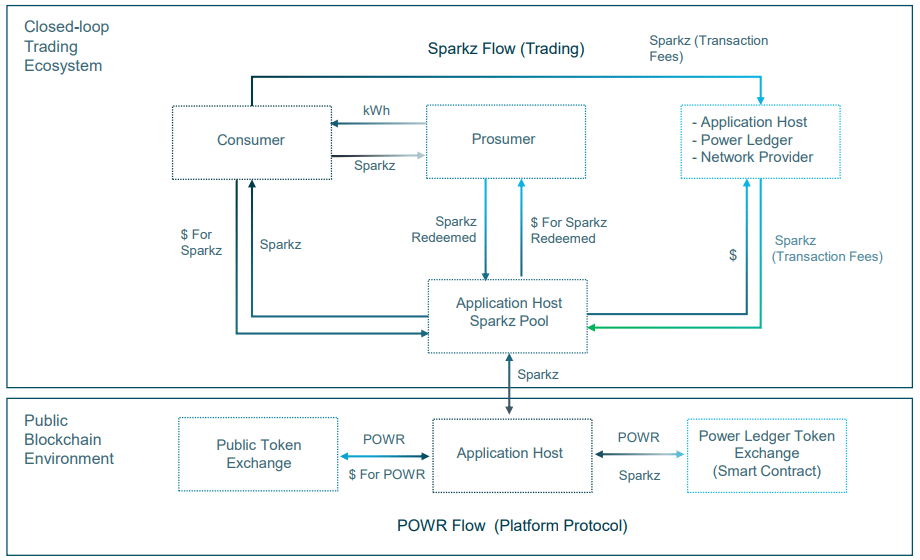
\includegraphics[width=1\textwidth]{Images/pl}
    \caption{Power Ledger Platform \cite{pl_home}.}
    \label{fig:pl}
\end{figure}

Through the Power Ledger application layer, prosumers and consumers can trade electricity directly with each other. This is done by initiating a smart contract. Meter readings are done by smart meters, and recorded in the blockchain, providing an audit trail for the participants. 

